\newpage
\section{Vorwort}
\subsection{Themenbegründung}
Die Entscheidung für das Brauen kam nicht sofort. Andere Ideen
 wie ein intelligenter Spiegel für das Badezimmer oder generell 
 ein Smarthome kamen uns in den Sinn. Wir hielten dies jedoch nicht
  für interessant genug. Wir dachten auch, dass wir etwas weg von der
   IT tun wollten, da wir täglich damit arbeiten. Wir haben versucht, 
   ein Thema zu finden, das uns Spaß macht, das neu und interessant ist und einen sozialen Aspekt hat.
Wir waren uns über das Brauen einig,
 da es etwas Neues ist. Etwas, das nicht jeder macht, 
 und das einen sozialen Aspekt hat, wenn man Brauer trifft und unser Bier mit Freunden und Familie testet.
\subsection{Persönliche Bezug - Callum Stringer}
Mein persönlicher Bezug zur Brauerei war mir ungemein wichtig. Ich habe vorher zu Hause ein wenig gebraut. 
Ich war ungeduldig erregt, meine Vorkenntnisse in einem Schulprojekt einzusetzen. Obwohl ich schon Erfahrung habe, habe ich schon eine ganze Weile nichts gebraut.
 Ich hoffe, dass dieses Projekt mein Interesse und meine Motivation, noch etwas Bier zu brauen, wieder wecken wird.
 \subsection{Persönliche Bezug - Fabrizio Franco}
 Meine Partner und ich habe uns zusammen für das Thema "Bier brauen" entschieden. Ich war für dieses Thema, weil ich selber
  gerne Bier trinke aber nicht genau weiss was in Bier enthalten ist oder wie überhaupt die Herstellung von Bier erfolgt. 
  Dazu noch weil mein Kollege Callum mir gut helfen kann, da er schon mal selber zuhause Bier gebraut hat und uns mit diesem 
  Experiment gut unterstützen kann. Es wundert mich zu wissen ob die Produktion von unterschiedlichen Sorten gleich ablauft oder 
  ob es bei bestimmten Sorten Abweichungen gibt. Mich interessiert auch zu wissen welche Unterschiede es bei der Herstellung von Bier
   zwischen Grossbrauereien wie Feldschlösschen und Kleinbrauereien gibt und wie die Preise für die verschiedenen Biersorten zustande 
   kommen. Hier in der Schweiz gibt es viele Kleinbrauereien und mich wundert es ob diese ein gewinnbringendes Geschäft oder eher eine
    Freizeit Beschäftigung sind. 
 Ich möchte mit diesem Projekt mein Wissen bezüglich Bier massiv erweitern da ich nur sehr weniger Erfahrung (abgesehen vom trinken) damit habe.
\subsection{\LaTeX\ }
Der Entschluss, \LaTeX\  als Werkzeug zur Dokumentenvorbereitung zu verwenden, wurde recht schnell gefasst. Wir haben \LaTeX\  bereits in
 der PVA verwendet. Es hat uns bei der Formatierung wirklich sehr geholfen und die Dinge einfach gehalten,
 so dass wir uns auf das Projekt konzentrieren konnten und uns keine Gedanken über das Herumfummeln mit Word machen mussten.
\\
Wir benutzten ein Git-Repository, um unsere Arbeit zu verfolgen, was es sehr einfach machte, als Team zusammenzuarbeiten. Da jeder in seinem Zweig arbeitete und die Arbeit abgeschlossen war,
 konnten wir8 eine Pull-Anfrage öffnen und alle Teammitglieder konnten sehen, ob etwas überprüft werden musste.
\subsection{Zusammenhang zwischen Klassen- und Gruppenthema}
Es war eine Herausforderung, eine Verbindung zwischen dem Bierbrauen und Neue Wege zu finden, aber man könnte es so betrachten, dass diese ganze Erfahrung, das Bierbrauen zu lernen, für uns ein neues Abenteuer und eine neue Erfahrung war. Man könnte also sagen, es war ein neuer Weg für uns als Gruppe.
Auf der anderen Seite haben Sie den Aspekt der Suche nach unseren Wurzeln, was unsere Vorfahren selbst gemacht haben, denn vor 100 Jahren konnten sie nicht in ihr lokales Geschäft gehen und Bier aus der Dose kaufen. Wir können uns vorstellen, dass sie es selbst getan haben. Wie wir es bei diesem Projekt getan haben
\newpage
\subsection{Ziel und Zielbegründung}
\newpage
\section{Einleitung}
\subsection{Einführung}
Brauen ist ein großes Thema. Wie man in der Mindmap sehen kann. Aber wir wollen uns konzentrieren und uns mit einigen wenigen spezifischen Themen befassen.
Zunächst einmal haben wir uns für das Brauen selbst entschieden, wir wollten diese Erfahrung selbst durchgehen. Wir haben uns entschieden, unser eigenes Bier mit Hilfe eines Bierkastens zu brauen. Dazu beschlossen wir auch, eine Verkostungsveranstaltung durchzuführen, um zu sehen, ob unser Bier gut ist. 
Das zweite Thema, das wir uns anschauen wollten, ist, ob es sich lohnt, ein eigenes Bier zu brauen. Dazu gehörten die Finanzen des Bierbrauens und ob es billiger geht. Dazu gehört auch, ob das Bier gut genug schmeckt. Es könnte billig sein, aber es könnte sich nicht lohnen, wenn der Geschmack schlecht ist.

\subsection{Mindmap}
Die Mind Map ist auf der nächsten Seite zu sehen, wir setzten uns hin und schrieben jede Idee auf, die uns in dieser Zeit in den Sinn kam. Danach nutzten wir diese als Planungshilfe und entschieden, welche Informationen und Themen wir untersuchen würden.
Die Hauptthemen, für die wir uns entschieden haben, sind die folgenden:
\begin{itemize}
   \item Umgebung - Besuch der Brauereien, Interviews/Besuch in der Brauereien
   \item Biersorten - Bei der Homebrew entscheiden wir um gewissen Biersorten
   \item Herstellung
   \item Finanziell
   \item Design
\end{itemize}
Die folgenden Ideen wurden aufgrund der zeitlichen Beschränkungen dieses Projekts nicht geprüft:
\begin{itemize}
   \item Wirtschaft sowie Kultur
   \item Alkohol
   \item Umfrage
   \item Geschichte
\end{itemize}
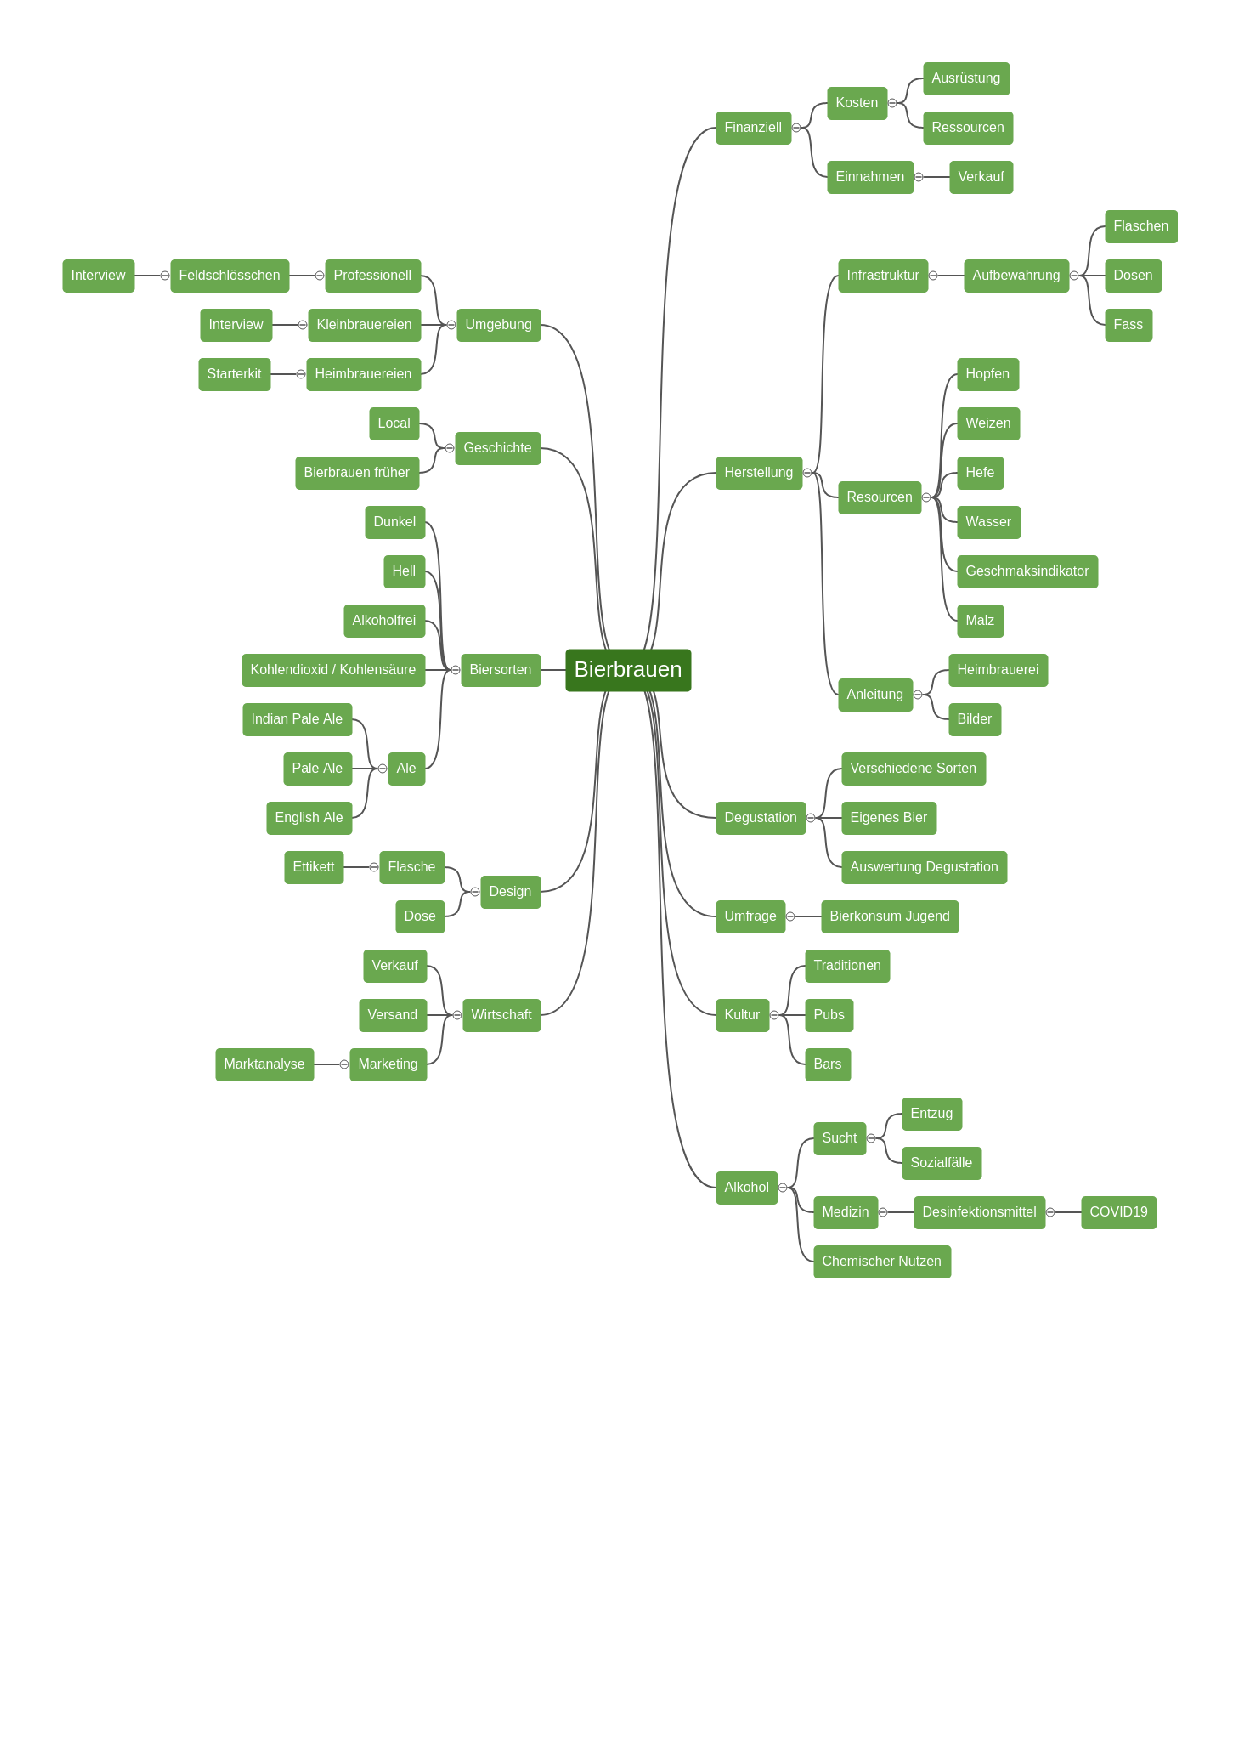
\includepdf{Mind-Map.pdf}

\subsection{Ziele} \label{introduction}
